\documentclass[a4paper, oneside, final]{scrartcl}
% import packages
\usepackage{scrpage2}
\usepackage{titlesec}
\usepackage{marvosym}
\usepackage{tabularx,colortbl}
\usepackage{fontspec}
\usepackage{multicol}
\usepackage[export]{adjustbox}
\usepackage{fontawesome}


% document settings
\defaultfontfeatures{Mapping=tex-text}
\titleformat{\section}{\large\scshape\raggedright}{}{0em}{}[\titlerule]
\pagestyle{scrheadings}
\addtolength{\voffset}{-0.5in} 
\addtolength{\textheight}{3cm}
\definecolor{Gray}{gray}{0.9}
\newcommand{\gray}{\rowcolor[gray]{.90}} 
\renewcommand{\headfont}{\normalfont}

% footer settings
\cofoot{\addfontfeature {LetterSpace=20.0} \fontsize{12.5}{17} \selectfont
{\faHome} reubencrimp.com 
{\Large\faGithub } github.com/rcrimp \\ 
{\faEnvelope} reubencrimp@gmail.com 
{\faPhone} (+64) 022 165 2992
% {\faSteamSquare} PhyterJet
}
\begin{document}



	%----------------------------------------------------------------------------------------
	% HEADER SECTION
	%----------------------------------------------------------------------------------------
	\noindent
   % \begin{minipage}{0.65\textwidth}
    \begin{center}	{\addfontfeature{LetterSpace=20.0}\fontsize{36}{36}\selectfont\scshape Reuben Crimp}
   \end{center}
   % \end{minipage}
	
   % \hfill
   % \begin{minipage}{0.3\textwidth}\raggedleft
   % 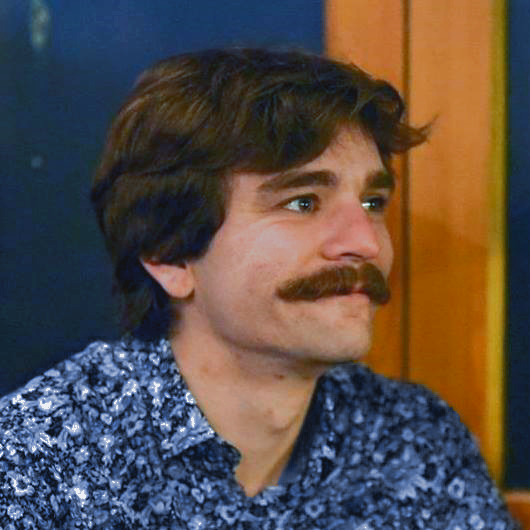
\includegraphics[width=.4\textwidth]{profile.png}
   % \end{minipage}

    %----------------------------------------------------------------------------------------
	%	EDUCATION
	%----------------------------------------------------------------------------------------
	\section{Education}
    
	\leftskip2em

    \begin{tabular*}{1.0\linewidth}{ll@{\extracolsep{\fill}}r@{\hspace{2em}}}
        \textbf{PGDipSci} & Computer Science, awarded with Distinction & 2016 \\
    	\textbf{BSc} & Major: Computer Science, Minor: Mathematics & 2013 --- 2015  \\
  	\end{tabular*}
    
    %----------------------------------------------------------------------------------------
	%	SKILLS
	%----------------------------------------------------------------------------------------
	 \section {Achievements} 
    
Scholarship for Academic Achievement in Science (University of Otago)   \hfill 2014 \\
ACM ICPC Programming Contest regional finals (UNSW, Sydney) \hfill 2014
     
     \section{Technical Skills}
      
	\begin{tabular}{ @{} >{\bfseries}l @{\hspace{4ex}} l }
    	Proficient & C, C\#, Java, Swift, Python, JavaScript\\
    	Familiar & C++, Haskell, SQL, PHP, GLSL, \LaTeX \\
    	Tools & vim, git, docker, Xcode, Visual Studio, Unity \\
        Libraries & opencv, opengl, nltk, three.js, Eigen, SDL \\
	\end{tabular}
    
    
    %----------------------------------------------------------------------------------------
	%	WORK EXPERIENCE
	%----------------------------------------------------------------------------------------
	\section{Research Experience}
    
    \begingroup\leftskip2em
   
   	\noindent
    \textbf{Research Assistant} --- Anatomy Department, University of Otago \hfill 2017 \hfill \\
	Developed software for annotating anatomical specimens, to be used for teaching.\\
    Supervised by Dr. Yusuf Cakmak.\\
    
    \noindent
    \textbf{Research Project} --- CompSci Department, University of Otago \hfill 2015 \hfill \\
	Developed virtual-reality software for chronic stroke rehabilitation.\\
    Supervised by Dr. Steven Mills and Dr. Holger Regenbrecht.\\
    
    \noindent
    \textbf{Summer Research Scholarship} --- CompSci Dept, University of Otago \hfill 2015 \hfill \\
	Designed and developed software for a lenticular auto-stereoscopic 3D display.\\
    Supervised by Dr. Geoff Wyvill.\\
    
    \noindent
    \textbf{Research Assistant} --- CompSci Department, University of Otago \hfill 2014 \hfill \\
	Determining the time complexity of network scheduling algorithms.\\
    Supervised by Dr.\ Haibo Zhang.\\
    
    \endgroup
    
    \section{Teaching Experience}
    \noindent	
    \textbf{Tutor} --- CompSci Dept, University of Otago \hfill 2017 --- \\
	Teaching undergraduate tutorials (lecture style), for 20-30 students. \\
    
    \noindent	
    \textbf{Tutor} --- Disability Information \& Support, University of Otago  \hfill 2015 --- \\
	One on one teaching on subject specific material. Computer science, maths, stats. \\
    
	\noindent	
    \textbf{Demonstrator} --- 	CompSci Dept, University of Otago \hfill 2014 --- \\
	Supervising CS undergrad computer labs, and assisting the students with their work. \\
    
    \section {Industry Employment}
    \noindent	
	\textbf{Intern iOS Developer} \hfill 2015 --- 2016 \\
	MixBit - Dunedin Office \\
	Worked in a small team developing iOS applications in swift. \\
    
    %----------------------------------------------------------------------------------------
	%	ACHIEVEMENTS
	%----------------------------------------------------------------------------------------
	\section{Projects \& Experience}
    
    \noindent        
	Developed virtual-reality software for chronic stroke rehabilitation.\\
	Using C\# and C++ with Unity and OpenCV. Involved heavy use of computer\\ vision techniques. Supervised by Dr.\ Steven Mills and Dr.\ Holger Regenbrecht.\\
    
	\noindent
	Designed and developed software for a lenticular auto-stereoscopic 3D display.\\ 
	Determined the internal optical properties of the display, then created several tools in C++, which generate and format 3D content. Supervised by Dr.\ Geoff Wyvill.\\

	\noindent
	Helped develop a command line shell for linux/OSX/Windows in C.\\
	A group project for university, where I was the main programmer, responsible for dealing with IO, pipes and processes on all three platforms.\\

	\noindent
	Other personal projects include CHIP-8 emulator, path tracer, raycaster, triangle rasterizer, and several games made with Unity/C\# and opengl/C.\\

	%\noindent
	%Competed in the 2014 ACM ICPC programming contest regional finals in Sydney.\\
    
	% exclude  academic record page
	\iffalse
      \pagebreak
      \section{Academic Record}
      Updated July 2015

      \begin{table}[h]
        \begin{tabular}{llllll}
        \rowcolor{Gray}
        \textbf{Year} & \textbf{Sem} & \textbf{Code} & \textbf{Course Name} & \textbf{Grade} & \textbf{Mark \%} \\
        %2015 & FY  & COSC490 & Honours Dissertation                            & --    & --      \\
        %2015 & S2  & COSC440 & Advanced Operating Systems                      & --    & --      \\
        %2015 & S2  & COSC450 & Computer Vision \& Graphics                     & --    & --      \\
        2015 & S1  & MATH342 & Modern Algebra                                  & B    & 73      \\
        %2015 & S1  & COSC410 & Logic for Artificial Intelligence               & --    & --      \\
        %2015 & S1  & COSC420 & Neural Networks                                 & --    & --      \\
             &     &         &                                                 &       &         \\
        2014 & FY  & COSC345 & Software Engineering                            & B+    & 75      \\
        2014 & S2  & COSC344 & Database Theory \& Applications                 & A+    & 96      \\
        2014 & S2  & COSC346 & Object-oriented Programming \& User Interfaces  & A     & 86      \\
        2014 & S1  & COSC341 & Theory of Computing                             & A+    & 93      \\
        2014 & S1  & COSC342 & Computer Graphics                               & A+    & 94      \\
        2014 & S1  & COSC343 & Artificial Intelligence                         & A     & 88      \\
        2014 & S1  & MATH272 & Discrete Mathematics                            & A-    & 81      \\
        2014 & SS  & COSC326 & Effective Programming                           & Pass  & --      \\
             &     &         &                                                 &       &         \\
        2013 & S2  & COMP212 & Advanced Web Development                        & A+    & 93      \\
        2013 & S2  & COSC242 & Algorithms \& Data Structures                   & A     & 87      \\
        2013 & S2  & COSC244 & Data-communications, Networks, Internet         & A+    & 93      \\
        2013 & S2  & MATH202 & Linear Algebra                                  & B+    & 75      \\
        2013 & S1  & COMP112 & Web Development \& Digital Media                & A+    & 93      \\
        2013 & S1  & COSC241 & Programming \& Problem Solving                  & A     & 87      \\
        2013 & S1  & COSC243 & Computer Architecture \& Operating Systems      & A     & 85      \\
        2013 & S1  & MATH170 & Mathematics 2                                   & C+    & 61      \\
             &     &         &                                                 &       &         \\
        2012 & S2  & BSNS106 & Information \& Communication                    & B     & 73      \\
        2012 & S2  & COMP160 & General Programming                             & A     & 85      \\
        2012 & S2  & ENGL127 & Effective Writing                               & B-    & 67      \\
        2012 & S2  & MATH160 & Mathematics 1                                   & A-    & 84      \\
        \end{tabular}
      \end{table}
    \fi
\end{document}